\documentclass[a4paper, 11pt]{article}

\usepackage[left=1.25in, right=1.25in, top=1.0in, bottom=1.0in]{geometry}
\usepackage[latin1]{inputenc}
\usepackage[T1]{fontenc}
\usepackage[francais]{babel}
\usepackage{fontspec}
\usepackage{amscd} 
\usepackage{amsfonts}
\usepackage{color}
\usepackage{fancyhdr}
\usepackage{listings}
\usepackage{float}
 \pagestyle{fancy}

%Entêtes et pieds de page
\fancyhead[C]{Génie Logiciel: Labo Final}
\fancyhead[L]{Schmidt Sébastien}
\fancyhead[R]{2014-2015}

\definecolor{mygreen}{rgb}{0,0.6,0}
\definecolor{mygray}{rgb}{0.5,0.5,0.5}
\definecolor{mymauve}{rgb}{0.58,0,0.82}

\lstset{ %
  backgroundcolor=\color{white},   % choose the background color; you must add \usepackage{color} or \usepackage{xcolor}
  basicstyle=\footnotesize,        % the size of the fonts that are used for the code
  breakatwhitespace=false,         % sets if automatic breaks should only happen at whitespace
  breaklines=true,                 % sets automatic line breaking
  captionpos=b,                    % sets the caption-position to bottom
  commentstyle=\color{mygreen},    % comment style
  deletekeywords={...},            % if you want to delete keywords from the given language
  escapeinside={\%*}{*)},          % if you want to add LaTeX within your code
  extendedchars=true,              % lets you use non-ASCII characters; for 8-bits encodings only, does not work with UTF-8
  frame=single,                    % adds a frame around the code
  keepspaces=true,                 % keeps spaces in text, useful for keeping indentation of code (possibly needs columns=flexible)
  keywordstyle=\color{blue},       % keyword style
  language=Octave,                 % the language of the code
  morekeywords={*,...},            % if you want to add more keywords to the set
  numbers=left,                    % where to put the line-numbers; possible values are (none, left, right)
  numbersep=5pt,                   % how far the line-numbers are from the code
  numberstyle=\tiny\color{mygray}, % the style that is used for the line-numbers
  rulecolor=\color{black},         % if not set, the frame-color may be changed on line-breaks within not-black text (e.g. comments (green here))
  showspaces=false,                % show spaces everywhere adding particular underscores; it overrides 'showstringspaces'
  showstringspaces=false,          % underline spaces within strings only
  showtabs=false,                  % show tabs within strings adding particular underscores
  stepnumber=1,                    % the step between two line-numbers. If it's 1, each line will be numbered
  stringstyle=\color{mymauve},     % string literal style
  tabsize=2                       % sets default tabsize to 2 spaces
}

%%%%%%%%%%%%%%%%%%%%%%%%%%%%%%%%%%%%%%%%%%%%%
%							Page de garde						 %
%%%%%%%%%%%%%%%%%%%%%%%%%%%%%%%%%%%%%%%%%%%%%
\makeatletter
\def\clap#1{\hbox to 0pt{\hss #1\hss}}%
\def\ligne#1{%
\hbox to \hsize{%
\vbox{\centering #1}}}%
\def\haut#1#2#3{%
\hbox to \hsize{%
\rlap{\vtop{\raggedright #1}}%
\hss
\clap{\vtop{\centering #2}}%
\hss
\llap{\vtop{\raggedleft #3}}}}%
\def\bas#1#2#3{%
\hbox to \hsize{%
\rlap{\vbox{\raggedright #1}}%
\hss
\clap{\vbox{\centering #2}}%
\hss
\llap{\vbox{\raggedleft #3}}}}%
\def\maketitle{%
\thispagestyle{empty}\vbox to \vsize{%
\haut{}{\@blurb}{}
\vfill
\vspace{1cm}
\begin{flushleft}
\usefont{OT1}{ptm}{m}{n}
\huge \@title
\end{flushleft}
\par
\hrule height 4pt
\par
\begin{flushright}
\usefont{OT1}{phv}{m}{n}
\Large \@author
\par
\end{flushright}
\vspace{1cm}
\vfill
\vfill
\bas{}{\@location, le \@date}{}
}%
\cleardoublepage
}
\def\date#1{\def\@date{#1}}
\def\author#1{\def\@author{#1}}
\def\title#1{\def\@title{#1}}
\def\location#1{\def\@location{#1}}
\def\blurb#1{\def\@blurb{#1}}
\date{\today}
\author{}
\title{}
\location{Amiens}\blurb{}
\makeatother
\title{Génie Logiciel: Labo Final}
\author{Schmidt Sébastien -  M18}
\location{Liège}
\blurb{%
Haute Ecole de la Province de Liège
}%

\begin{document}
\maketitle

\tableofcontents
\newpage

\section{Technologies utilisées}
	Pour ce projet final de génie logiciel, j'ai utilisé quelques technologies que je vais me charger d'expliquer dans cette section. Certaines étaient demandées et d'autres non, j'expliquerai mes choix quant à l'utilisation de ces technologies.
	\subsection{GitHub}
		C'est un service web d'hébergement et de gestion de développement de logiciels, utilisant le logiciel de gestion de versions Git. Il permet la gestion de version décentralisé. Cela fonctionne par commit, chaque personne pouvant travailler sur ce projet possèdera une version locale. Les changements apporté à cette version seront alors <<commité>> sur le serveur où chacun devra <<pull>> les données régulièrement pour avoir les dernières versions. Il est également possible de revenir en arrière vers un précédent commit lorsque l'application était stable. C'est principalement pour cette raison que j'ai utilisé un répertoire Git public. 
		
	\begin{figure}[!h]
		\centering
		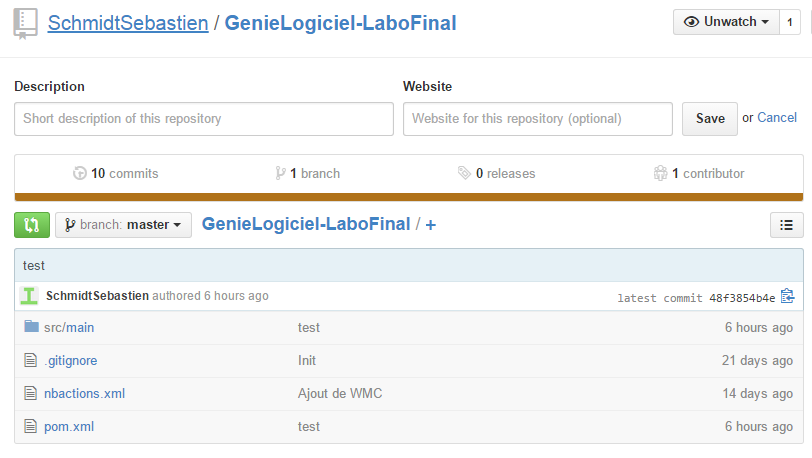
\includegraphics[scale=0.6]{Images/git.png}
		\caption{Le repository de l'application finale de génie logiciel sur GitHub}
	\end{figure}
	
	\subsection{Maven}
		Maven est un outil prévu pour la gestion et l'automatisation de production des projets logiciels Java. L'objectif recherché est comparable au système Make sous Unix : produire un logiciel à partir de ses sources, en optimisant les tâches réalisées à cette fin et en garantissant le bon ordre de fabrication. De cette façon quand on met en projet sur un Git, tous les fichiers propres à la configuration de l'IDE ne sont pas pris en compte. Il est semblable à l'outil Ant, mais fournit des moyens de configuration plus simples, eux aussi basés sur le format XML. Maven utilise un fichier de configuration POM (Project Object Model) permettant de décrire un projet logiciel et ses dépendances avec des modules externes (comme javaparser par exemple) et l'ordre à suivre pour sa production.
		
		\subsubsection{pom.xml}
		\textcolor{red}{TODO}
	
	\subsection{JUnit}
		Pour effectuer le testing de l'application, j'ai utilisé le framework JUnit dans le but de réaliser des tests unitaires en programmation Java.
	
	\subsection{Jacoco}
		Pour réaliser la couverture des tests, j'ai utilisé un outil permettant la couverture de code comme Jacoco qui est plus adapté aux tests d'intégration que Cobertura. Il est intégré au projet sous forme de dépendance via Maven. Toutes ses informations sont donc placées dans le pom.xml. Le plugin JaCoCo va générer la configuration de l’agent pour lancer les tests.
		
	\begin{figure}[!h]
		\centering
		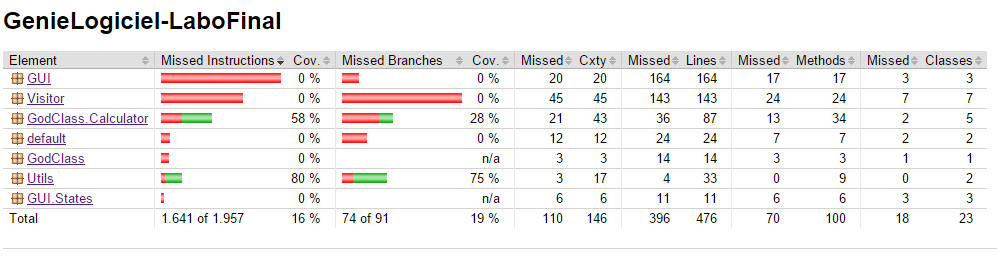
\includegraphics[scale=0.6]{Images/jacoco.png}
		\caption{La couverture du code à un état peu avancé du projet}
	\end{figure}
	
	\subsection{Jenkins}
		Outil d'intégration continue qui est en réalité un fork de l'outil Hudson. Il s'interface avec des systèmes de gestion de versions tels que CVS, Git et Subversion, et exécute des projets basés sur Apache Ant et Apache Maven. Ce serveur permet donc de configurer un projet en fonction des dépendances dont on a besoin. Pour ce projet, j'ai configuré le serveur pour aller récupérer les données d'un projet Maven sur un repository Git tout en effectuant la couverture du code avec Jacoco. Tous ces outils sont par conséquent configuré dans les paramètres du serveur. Un build s'effectue une fois par jour.
	
\section{Diagramme de classes}
	Sur la figure \ref{diag1} on peut voir que j'ai en fait un objet <<Calculator>> qui va encapsuler les différentes classes qui permettront de calculer les métriques. Elle possède par conséquent quatre classes:
	\begin{description}
		\item[GeneralCalculator :] Cette classe aura la tâche de stocker les données générales à l'application comme le nombre de lignes qu'une classe possède, son nom ou encore son nombre de méthodes.
		\item[WeightedMethodCountCalculator :] Cette classe va compter le nombre de branchement d'une classe et on obtiendra le métrique calculé par la méthode de McCabe. Moins il y a de branchements, moins la classe sera complexe, mieux ce sera.
		\item[ClassCohesionCalcuator :] Cette classe mesure la cohésion d'une classe en fonction de ses variables membres. Plus celles-ci sont utilisées dans différentes méthodes, plus la classe sera cohérente.
		\item[AccessToForeignDataCalculator :] Cette classe mesure le nombre de classes externe qui seront utilisées via ses attributs ou ses accesseurs. De nouveau moins il y en aura, mieux ce sera.
	\end{description}
	
	\begin{figure}[!h]
		\centering
		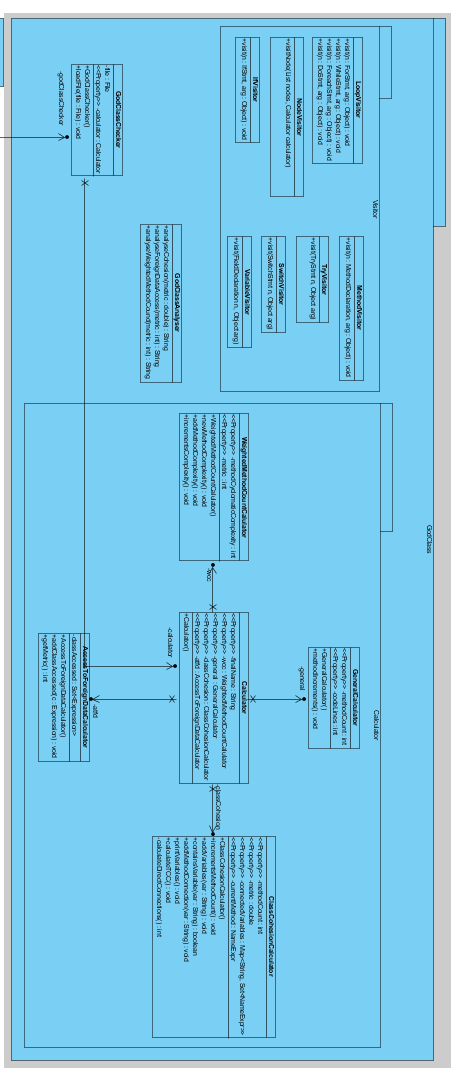
\includegraphics[scale=0.8]{Images/ClassDiagram1.png}
		\caption{Première partie du diagramme de classe}
		\label{diag1}
	\end{figure}
	
	Toutes ces classes auront donc les métriques calculés. C'est la classe <<GodClassChecker>> qui possèdera une instance de la classe <<Calculator>>. Comme le java parser utilise des visitors pour parcourir l'ensemble de l'arbre AST construit, je passerai cette classe en paramètre et les différents métriques seront calculés au fur et à mesure que la classe sera parsée. Quand le parsing sera terminé, il me suffira ensuite d'utiliser la classe <<GodClassAnalyser>> qui comme son nom l'indique va analyser les différents résultats obtenus. Elle possède trois méthodes: une pour chaque métrique à analyser. Chacune d'entre elle prendra le métrique correspondant et sortira une petite analyse afin de savoir si la classe a bien été conçue.
	
	Comme dit précédemment, le javaparser utilise les visiteurs pour parcourir l'ensemble de la classe. Chacun des visiteurs que j'ai créé va hériter d'une classe VoidVisitorAdapter. Celle-ci contiendra une série de méthodes adaptées pour parcourir chaque type de lignes. Les visiteurs utilisés:
	\begin{description}
		\item[MethodVisitor :] Il va visiter l'ensemble de chaque méthode et va pouvoir ensuite appeler le visiteur correspondant au type de <<statement>> rencontré.
		\item[NodeVisitor :] C'est lui qui, appelé par le <<MethodVisitor>> va pouvoir redirigé le parser vers le bon visiteur
		\item[LoopVisitor :] Celui-ci, comme son nom le laisse penser, permet de parcourir les différents types de boucle. Il possède trois méthodes: une pour les boucle while, une boucle pour les boucles for et une pour les boucle do.
		\item[TryVisitor :] Ce visiteur va pouvoir parcourir les blocs Try catch.
		\item[SwitchVisitor :] Va permette de parcourir les switchs et ses différentes case.
		\item[VariableVisitor :] On arrive à la fin de l'arbre, il ne reste plus que les variables à analyser, c'est lui qui va s'en occuper.
	\end{description}
	
	\begin{figure}[!h]
		\centering
		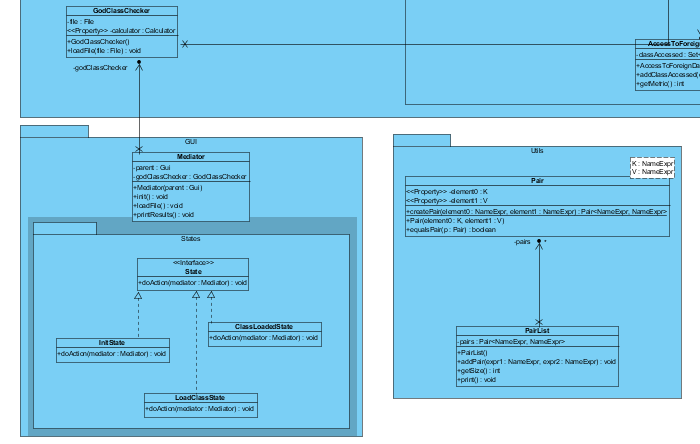
\includegraphics[scale=0.8]{Images/ClassDiagram2.png}
		\caption{Deuxième partie du diagramme de classe}
		\label{diag2}
	\end{figure}
	
	Sur la seconde partie du diagramme de classe (figure \ref{diag2}, on peut voir l'utilisation d'un médiateur, celui-ci permet en réalité de centraliser les interactions entre les différents composants de l'interface graphique. Il aura en variable membre une instance d'un <<GodClassChecker>> et utilisera le <<GodClassAnalyser>> pour analyser et afficher des messages sur ces métriques calculés.
	
	On peut également voir un package <<States>> qui comprendra trois états. Ceux-ci reflètent l'état dans lequel se trouve l'application:
	\begin{description}
		\item[InitState :] Etat initial de l'application, des actions effectuées qu'une seule fois ce feront à ce moment.
		\item[LoadClassState :] Une nouvelle classe est chargée en mémoire, il faut la charger et la parser.
		\item[ClassLoadedState :] La classe a été parsée, il faut maintenant afficher les résultats et les calculer.
	\end{description}
	
\section{Diagramme pour les différents packages}
	\begin{figure}[!h]
		\centering
		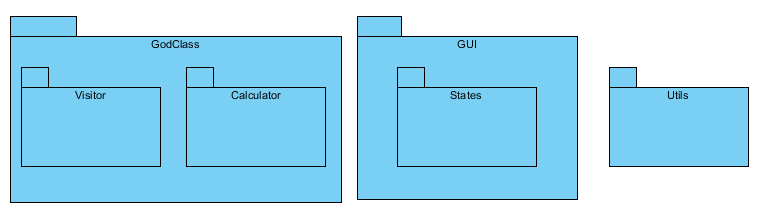
\includegraphics[scale=0.8]{Images/packages.png}
	\end{figure}
	
	J'ai divisé mon application en trois packages principaux: 
	\begin{enumerate}
		\item Un package <<GodClass> qui encapsulera un nouveau  package <<Visitor>> et un autre <<Calculator>>.
		\item Un package <<GUI>> qui englobera un autre package <<States>>
		\item Et enfin un package <<Utils>> dans lequel je placerai les classes utiles utilisées dans d'autres classes.
	\end{enumerate}
	
\section{Diagramme de séquence}

	Pour ce diagramme de séquence, je vais faire abstraction des classes d'état, des classes représentent les différents métriques (ils seront tous représentés par la classe <<Calculator>>) ainsi que la classe GUI gérant l'interface graphique. On commence avec le médiateur qui appelle une méthode du <<GodClassChecker>> pour charger la classe en mémoire. On passe ensuite dans un premier visiteur qui est celui de la méthode et elle va appeler plusieurs méthodes de la classe <<Calculator>>. On va ensuite parcourir chaque noeuds de la méthode dans une boucle: il y aura deux cas d'utilisation:
	\begin{enumerate}
		\item Si le noeud est une variable, on va dans ce cas là ajouter des informations concernant ce que le parser est train de lire. Ces informations seront enregistrées via des appels de méthodes de la classe <<Calculator>>.
		\item Si le noeud est un statement comme un if, une boucle, un bloc try, ... il faudra incrémenter la complexité cyclomatique du caclulator. Pour chaque noeud de celui-ci on reparcourera la boucle.
	\end{enumerate}
	
	Une fois cette boucle terminée, il reste à calculer le WMC de et d'afficher les différents résultats obtenus.

	\begin{figure}[!h]
		\centering
		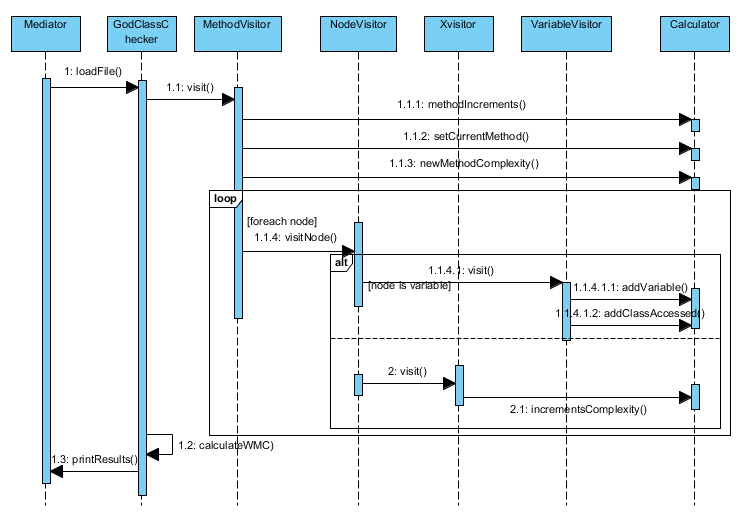
\includegraphics[scale=0.8]{Images/seq.png}
		\caption{Diagramme de séquence de la principale fonctionnalité de l'application}
	\end{figure}

\section{Choix de conception}
	Au niveau de la conception, j'ai utilisé trois patrons de conception vus au cours: Le state pattern, le mediator pattern et le visitor pattern.
	
	Concernant l'interface graphique de l'application, j'ai utilisé un médiateur afin d'encapsuler toutes les interactions graphiques. Lorsqu'un logiciel est composé de plusieurs classes, les traitements et les données sont répartis entre toutes ces classes. Plus il y a de classes, plus le problème de communication entre celles-ci peut devenir complexe. En effet, plus les classes dépendent des méthodes des autres classes plus l'architecture devient complexe. Cela ayant des impacts sur la lisibilité du code et sa maintenabilité dans le temps. Le modèle de conception Médiateur résout ce problème. Pour ce faire, le Médiateur est la seule classe ayant connaissance des interfaces des autres classes. Lorsqu'une classe désire interagir avec une autre, elle doit passer par le médiateur qui se chargera de transmettre l'information à la ou les classes concernées. Bien qu'il n'y ait pas énormément de classes dans cette application, si par la suite on désire rajouter plus de classes faisant encore plus d'interactions, il n'y aurait pas de problème, elles passeraient toutes par ce médiateur. Par exemple pour charger une fichier java, ce sera le médiateur qui va s'en charger, il ne reste plus qu'à appeler la méthode du médiateur dans l'interface graphique.
	
	\lstinputlisting[language=Java, firstline=38, lastline=56]{../src/main/java/GUI/Mediator.java}
	
	Comme l'application peut avoir plusieurs états, j'ai élaboré une hiérarchie d'états correspondant chacun à un état dans lequel l'application peut se trouver. Par conséquent, l'interface graphique possèdera une variable membre correspondant à un état, il suffira ensuite de créer une nouvelle instance de l'état en question et d'appeler sa méthode doAction() qui permettra de remplir le rôle de cet état.
	
	\lstinputlisting[language=Java, firstline=222, lastline=228]{../src/main/java/GUI/Gui.java}
	
	La méthode doAction de l'état LoadClass ne fera qu'appeler la méthode du médiateur permettant de charger la classe.
	
	\lstinputlisting[language=Java, firstline=14, lastline=21]{../src/main/java/GUI/States/LoadClassState.java}
	
	J'ai ensuite utilisé les visiteurs pour parcourir l'ensemble du fichier. Dans un premier temps la classe <<MethodVisitor>> est appelée.  Celle-ci appellera par après la classe <<NodeVisitor>> qui permettra d'utiliser correspondant au cas qui sera concerné.
	\lstinputlisting[language=Java, firstline=35, lastline=37]{../src/main/java/GodClass/Visitor/MethodVisitor.java}
	
	Dans la classe <<NodeVisitor>>, on va passer en revue tous les types de <<Statement>> que l'on peut rencontrer et chacun des cas correspondra à une action différente.
	\lstinputlisting[language=Java, firstline=32, lastline=51]{../src/main/java/GodClass/Visitor/NodeVisitor.java}
	
	Par exemple, si le <<statement>> que l'on examine est une boucle, on va y faire le traitement suivant:
	\begin{enumerate}
		\item Récupère l'objet passé en paramètre permettant de sauvegarder les résultats
		\item Si la condition est une condition binaire, on incrémente la complexité de McCabe
		\item On la réincrémente une seconde fois car la boucle ajoute une branche dans l'arbre
		\item On récupère ensuite l'ensemble de noeuds et on les reparcours grâce au <<NodeVisitor>>, on repart ensuite pour un tour et ainsi de suite jusqu'à la fin de l'application
	\end{enumerate}
	\lstinputlisting[language=Java, firstline=25, lastline=39]{../src/main/java/GodClass/Visitor/LoopVisitor.java}
	
\section{Techniques de tests}

\section{Cas concrets d'utilisation}

\end{document}